\documentclass[main.tex]{subfiles}
\begin{document}

\section{Achieving interpretibaility in compositional models} % 3pp
\label{sec:nmn-interpret}

\subsection{Introduction}
Models that can read text and reason about it in a particular context (such as an image, a paragraph, or a table) have been recently gaining increased attention, leading to the creation of multiple  datasets that require multi-step reasoning in both the visual and textual domain \cite{clevr-2017,nlvr-suhr-2017,complexweb-talmor-2018,hotpotqa-2018,nlvr2-suhr-2018,gqa-hudson-2019,drop-2019}.
Consider the example in Figure~\ref{fig:03-intro} from \nlvr{}: a model must understand the compositional sentence in order to then ground \emph{dogs} in the input, count those that are \emph{black} and verify that the count of all dogs in the image is equal to the number of black dogs.


%
\begin{figure}[bh!]
    \centering
    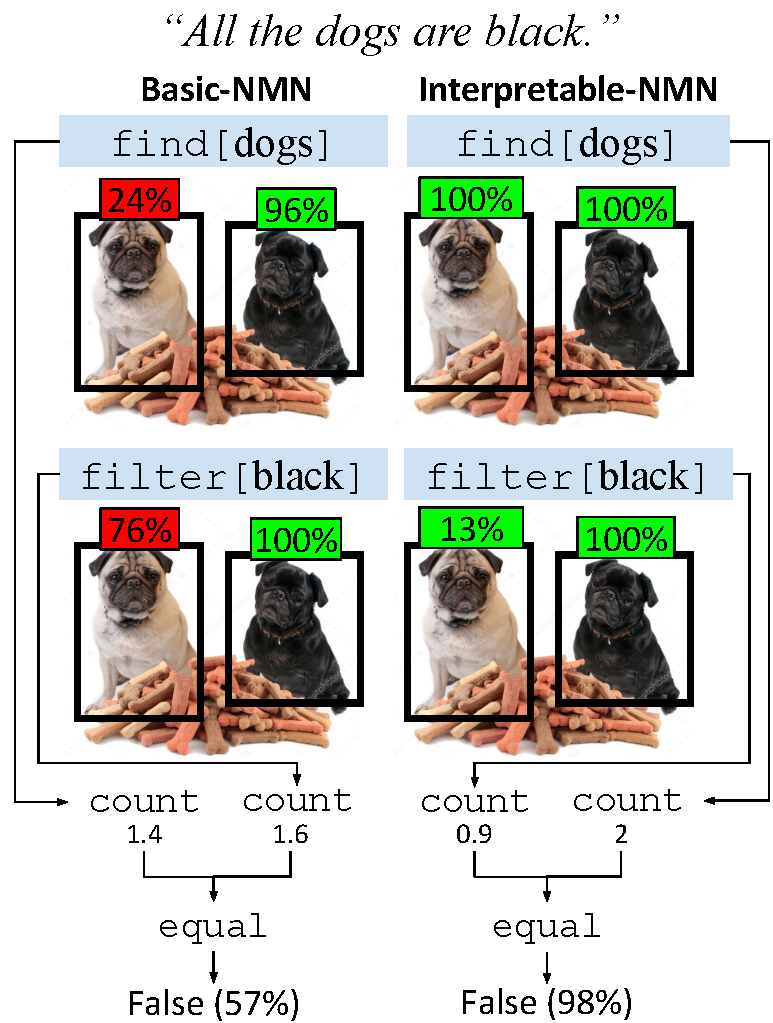
\includegraphics[width=62mm]{03-intro.pdf}
    \caption{An example for a visual reasoning problem where both the Basic and Interpretable NMNs produce the correct answer.
    The Basic NMN, however, fails to give meaningful intermediate outputs for the \texttt{find} and \texttt{filter} modules, whereas our improved interpretable-NMN assigns correct probabilities in all cases. Boxes are green if probabilities are as expected, red otherwise.}
    \label{fig:03-intro}
\end{figure}


Both models that assume an intermediate structure \cite{nmn-2016,jiang-nmn-2019} and models without such structure~\cite{lxmert-hao-2019,mtmsn-2019,compositional-min-2019} have been proposed for these reasoning problems.
While good performance can be obtained without a structured representation, an advantage of structured approaches is that the reasoning process is more \emph{interpretable}. For example, a structured model can explicitly denote that there are two \emph{dogs} in the image, but that one of them is not \emph{black}. Such interpretability improves our scientific understanding, aids in model development, and improves overall trust in a model.

\begin{figure}[tbh]
\centering
    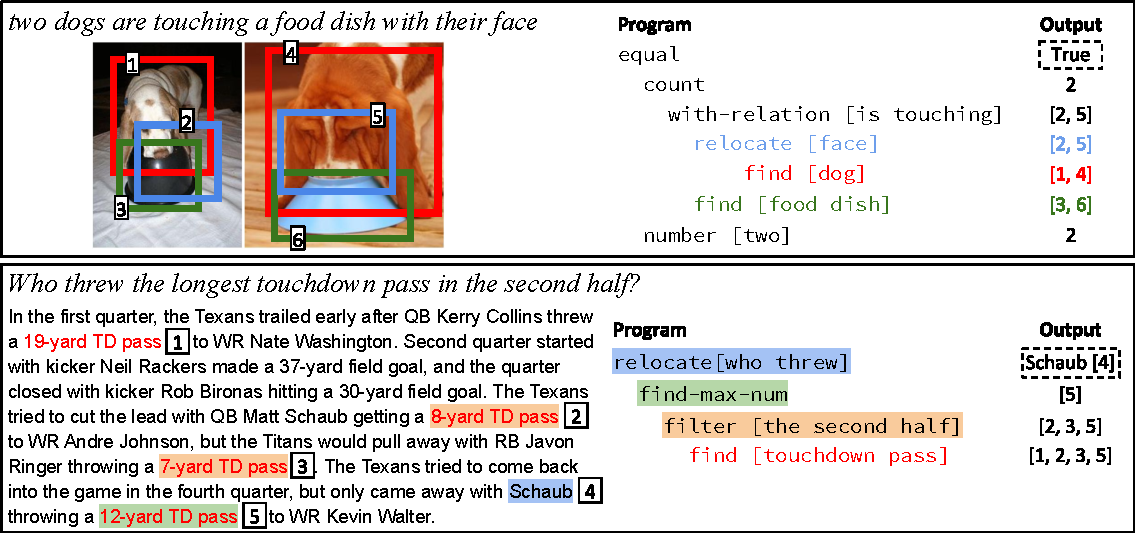
\includegraphics[width=0.9\textwidth]{03-combined.pdf}
    \caption{An example for a mapping of an utterance to a gold program and a perfect execution in a reasoning problem from \nlvr{} (top) and \drop{} (bottom).}
 \label{fig:03-nmn-example}
\end{figure}

Neural module networks (NMNs;~\newcite{nmn-2016}) parse an input utterance into an executable program composed of learnable modules that are designed to perform atomic reasoning tasks and can be composed to perform complex reasoning against an unstructured context. NMNs are appealing since their output is interpretable; they provide a structured parse of the utterance and also the intermediate outputs performed to reach the final answer.
However, because module parameters are typically learned from end-task supervision only, it is possible that the model will solve the task, but the modules will not perform the reasoning steps as intended. In Figure~\ref{fig:03-intro}, a \emph{basic NMN} predicts the correct answer \texttt{False}, but does not correctly locate one of the \emph{dogs} in the image. This is undesirable, since the motivation for NMNs in this case is interpretability.
While recent work~\cite{explainablenmn-hu-2018,jiang-nmn-2019} has shown that one can obtain good performance when using NMNs, interpretability was mostly evaluated through qualitative analysis, rather than systematically evaluating the intermediate outputs of each module.

We provide three primary contributions regarding interpretability in NMNs.
First, we propose the concept of \emph{module-wise interpretability} -- a systematic evaluation of individual module performance that judges whether they have learned their intended operations, and define metrics to quantify this for both visual and textual reasoning (\S\ref{ssec:measure}).
Second, we provide strategies for improving module-wise interpretability in NMNs (\S\ref{ssec:interpret}).
Specifically, (a) we demonstrate how module architecture affects interpretability,
(b) propose supervising module outputs with either a proxy task or heuristically generated data, and (c)
show that providing modules with uncontexualized token representations improves interpretability.

Empirically, we show on both \nlvr{}~\cite{nlvr2-suhr-2018} and \drop{} \cite{drop-2019} that training a NMN using end-goal supervision, even using \emph{gold programs}, does \emph{not} yield module-wise interpretability, i.e., the modules do not perform their intended reasoning task.
We show that the different strategies proposed in this work improve interpretability to a great extent, sometimes at the cost of modest degradation in end-task performance.
Figure~\ref{fig:03-intro} shows an example where our approach (\emph{Interpretable-NMN})
results in much more sensible module outputs as compared to the \emph{Basic-NMN}.


\subsection{Module-wise Interpretability}
\label{ssec:measure}
Neural module networks facilitate interpretability of their predictions by describing the reasoning steps as the program modules, and providing the intermediate outputs of those steps during execution.
For example, in Figure~\ref{fig:03-nmn-example}, all reasoning steps taken by both the Visual-NMN and Text-NMN are interpretable.
However, because module parameters are learned from an end-task, there is no guarantee that the modules will learn to perform their intended reasoning.
Work on NMNs thus far~\cite{explainablenmn-hu-2018,jiang-nmn-2019} has overlooked systematically evaluating interpretability, performing only qualitative/subjective analysis in this regard.

We introduce the concept of \textit{module-wise interpretability}, aimed at providing an evaluation of module performance in a trained NMN.
Module-wise interpretability evaluates whether each module has correctly learned its intended operation by judging the correctness of the \emph{intermediate} module outputs.
For example, in Figure~\ref{fig:03-nmn-example} (top), a model would be judged module-wise interpretable if the outputs of all the modules, \texttt{find}, \texttt{relocate}, and \texttt{with\_relation}, are correct.

Along with an interpretability score for each module separately, we compute its micro-average, i.e., an overall interpretability score.
We provide gold programs when evaluating interpretability, to not conflate  interpretability with parser accuracy.

\paragraph{Measuring interpretability in Text-NMN}
Each module in Text-NMN produces a distribution over passage tokens which represents the selected spans in a soft manner.
In order to measure module-wise interpretability of Text-NMN, we
annotated the set of spans that should be output by each module in the gold program (see \S\ref{ssec:exp-setup} for details).
Ideally, modules like \texttt{find}, \texttt{filter}, etc., should predict high probability for tokens that appear in the gold spans and \textit{zero} probability for other tokens. For example, the relevant spans for each module are shown in Figure~\ref{fig:03-nmn-example} (bottom).

Concretely, we use a metric akin to cross-entropy loss to measure the deviation of the predicted module output $p_{\text{att}}$ from the gold spans  $S~=~[s_{1}, s_{2}, \ldots, s_{N}]$. Here each span $s_{i} = (t^{i}_{\text{start}}, t^{i}_{\text{end}})$ is annotated as the start and end tokens.
Interpretability for a module is measured by:
\begin{equation*}
    I = - \sum_{i=1}^{N}  \Bigg(\log \sum_{j = t^{i}_{\text{start}}}^{t^{i}_{\text{end}}} p_{\text{att}}^{j} \Bigg).
\end{equation*}
Here, lower cross-entropy corresponds to better interpretability of a module.

\paragraph{Measuring interpretability in Visual-NMN}
Simiarly, we define a quantitative meausure of interpretability in Visual-NMN based on the overlap between gold and predicted bounding-boxes that should be output by each module in the program. For brevity, we omit the details and refer the reader to the paper~\missingcite{}.


\subsection{Improving Interpretability in NMNs}
\label{ssec:interpret}
Module-wise interpretability is affected by various factors; the choice of modules and their implementation, use of auxiliary supervision, and the use of contextual utterance embeddings. We discuss ways of improving interpretability of NMNs across these dimensions.

\subsubsection{Choice of modules}



\biblio

\end{document}
